\chapter{Introduction} % Main chapter title
\label{Chapter1} % For referencing this chapter elsewhere, use \ref{Chapter1}

\noindent 
\section{Literature review}
\noindent
In medical studies, the paradigm of survival analysis is used to determine outcome events based on patient survival data. Due to the censoring complexities and high dimensionality these datasets often entail, formal statistical approaches have been developed  chronologically, each iteration improving and building upon fundamental statistical properties of survival data and the underlying result interpretation. 
\subsection{Background} 
\noindent
Survival analysis is used to examine the time until the occurrence of an event like disease relapse. A major challenge in this area is handling censored data, where the event information is incomplete. Censoring can be of different types: right-censored data is when the event has not occurred by the end of the observation period; left-censored data is when the event occurred before the study began; and interval-censored data is when the event occurred between two observed times. In order to analyse such data, statistical methods have been developed. Non-parametric methods like the Kaplan-Meier estimator and the Logrank test do not assume any specific distribution for the time-to-event data, making them robust against mis-specifications of the event-time distribution. Parametric methods like the Exponential and Weibull models assume a known distribution that models the time-to-event data. They are typically more precise, at the risk of introducing bias when the assumed distribution is wrong. The Proportional Hazards Model, which can be used in both semi-parametric (Cox model) and parametric forms, is employed to estimate the hazard ratio, which is a measure of effect size regarding the time to event. An example of this is found with the study [1] could be that of analysing motion-sickness data, where survival functions are estimated and treatments are compared. For instance, studies may compare the time until onset of motion sickness under different conditions to assess treatment effectiveness.

Traditional statistical methods require explicit programming and often suffer from user bias in variable selection. Machine Learning (ML) operates under a paradigm where algorithms autonomously identify patterns in large data sets, which potentially increases accuracy and efficiency. [2] Show that, the literature on ML in orthopaedics, predominantly composed of preliminary studies, frequently lacks depth in addressing complex ML concepts and falls short in providing comprehensive frameworks for result interpretation. Deep Learning, a prominent subset of ML, utilises neural networks to process both structured and unstructured data, enhancing the capability to handle diverse data types like images and texts. [2] 
[3] Also show out of their methodical study selection process that only a handful of studies have attempted such comparisons at an acceptable standard, while most studies focus predominantly on machine learning techniques neglecting the broader spectrum of statistical methods. Furthermore [3] point out authors often omit interaction terms and non-linear covariate effects which are essential components for enhancing model robustness and accuracy. The predominance of studies failed to relax the proportional hazards assumption which underscores a critical oversight in adapting models to more complex datasets. [3] show that there is a need for comprehensive methodological improvements and enhanced reporting standards to ensure reproducibility and a fair assessment of method capabilities[3]
\begin{figure}
	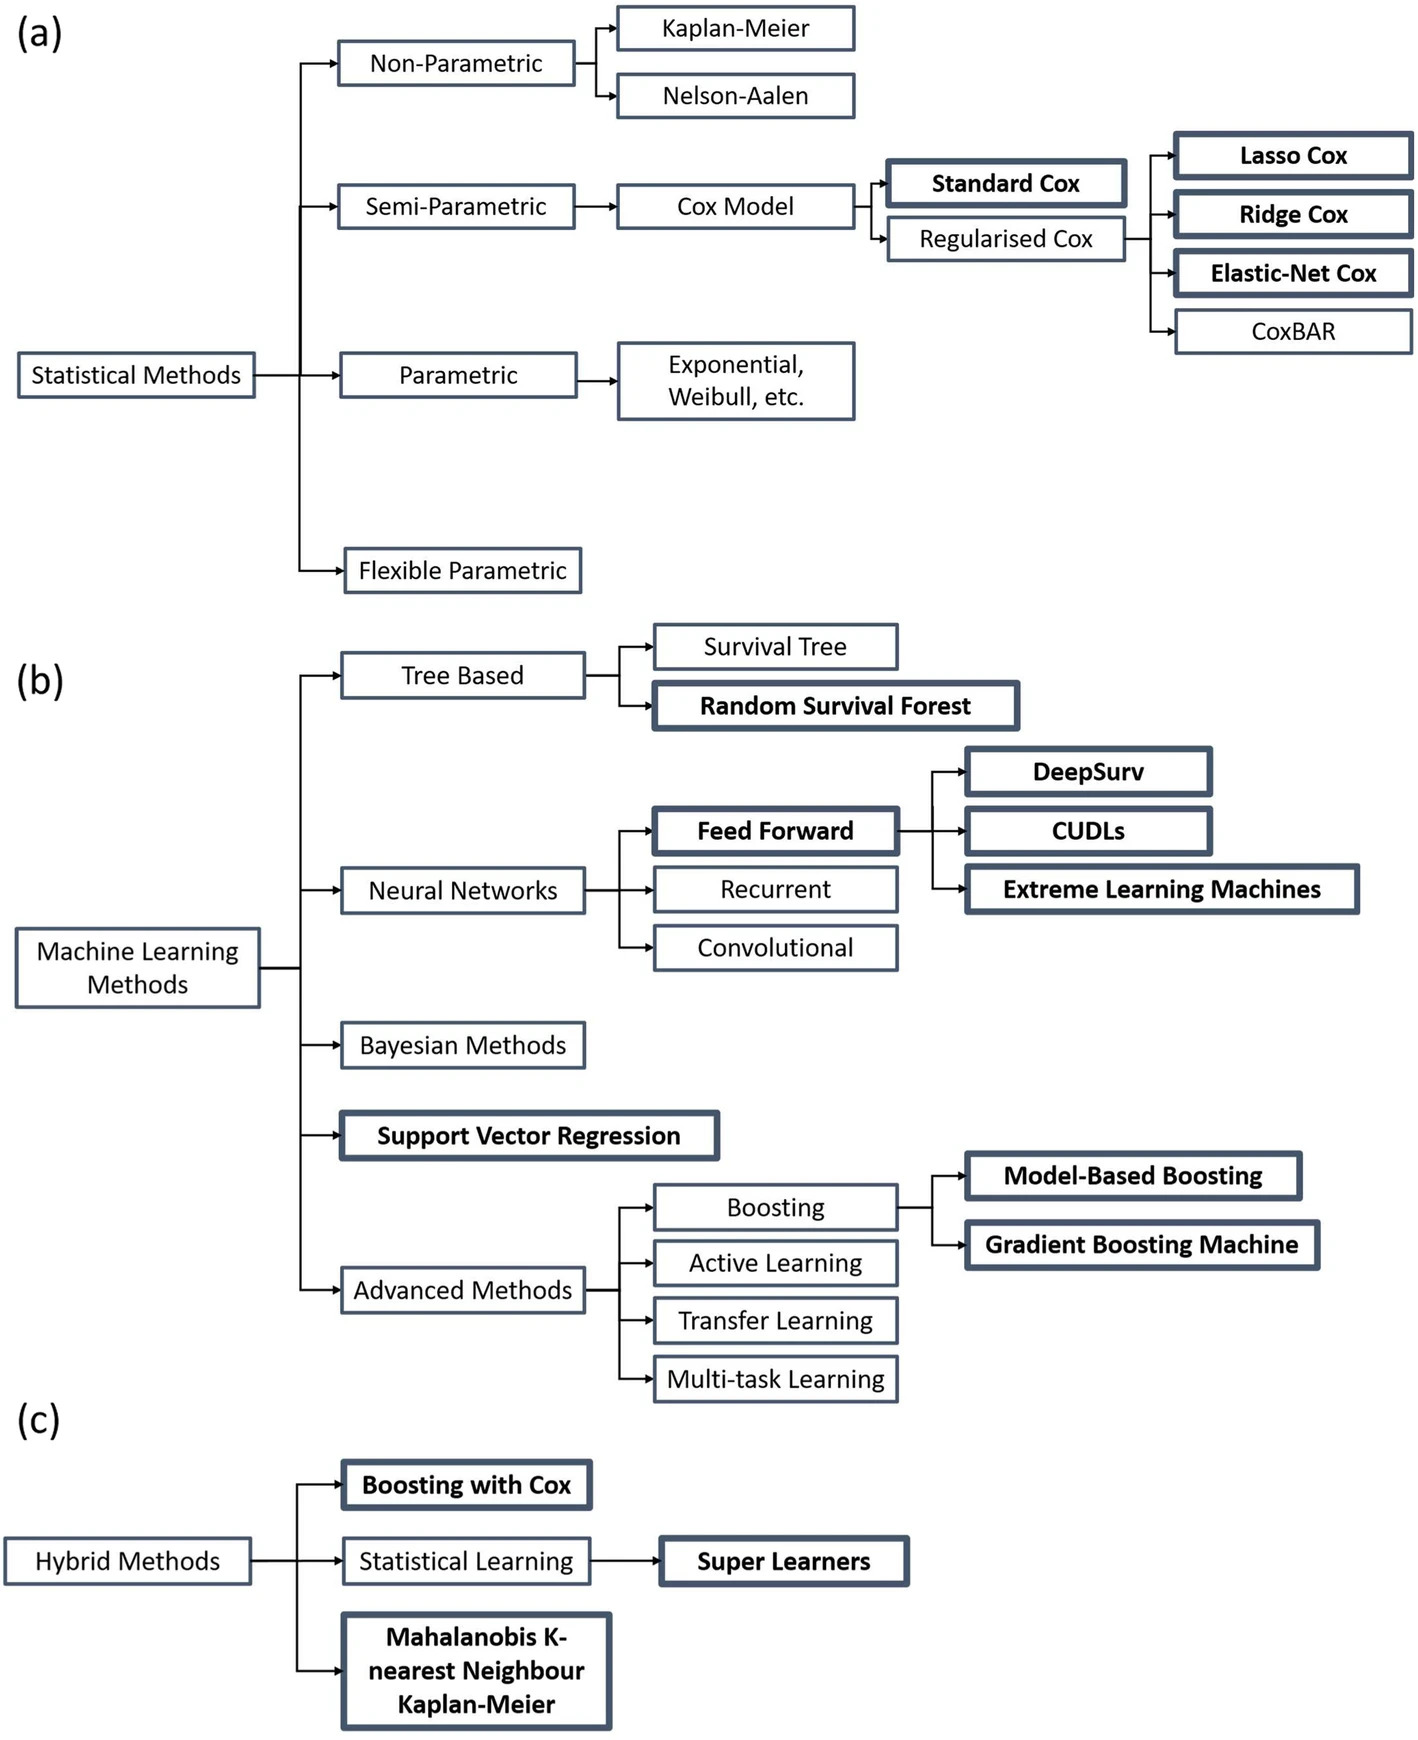
\includegraphics[scale=0.3]{Figures/screenshots/ML_STATS_MODELS.jpg}
	\caption{Shows the breakdown of methods analysis preformed by \parencite*{} during a method review. The Study ran a literature selection process based on qualitative and quantitative metrics of methodology used in studies.}
\end{figure}
\subsubsection{Important issues in comparative simulation studies}

\noindent 
Simulation studies are a crucial statistical tool used for evaluating and comparing different statistical methods, particularly when analytic solutions are hard or impossible to achieve. These studies generate data through pseudo-random sampling from known probability distributions, enabling researchers to empirically test the behaviour of statistical methods under varied scenarios. Common uses include validating new statistical methods, ensuring accuracy in mathematical models and code, and comparing the effectiveness of various approaches. Particularly in medical statistics, simulation studies help in designing experiments, determining sample sizes, and estimating power under specific assumptions about data generation [4]. Despite their widespread use, many statisticians face challenges in properly conducting simulation studies due to a lack of understanding and experience [4]. Common issues include inadequate design and reporting that lead to uncritical acceptance of results. This lack of rigour can result in misleading conclusions, for example the variability introduced by different sets of random numbers in Monte Carlo simulations that is sometimes ignored.

[3] Found a notable scarcity of quality comparative research between statistical and machine learning methods. Predominantly, these studies focus on machine learning techniques while traditional statistical methods are often neglected. 

For instance, it was common for some authors to overlook the inclusion of interaction terms and non-linear covariate effects in the Cox model as well as time-dependent effects which are key elements for effectively handling complex datasets.

The reporting standards of the reviewed studies were also generally poor. Important details such as data-generating mechanisms (DGMs), estimands, and method implementations are frequently underreported, which impedes the reproducibility of the research and the ability to conduct fair comparisons between methods. 

[3] Also pointed out that a significant bias could be observed in the selection of DGMs, which tend to favour machine learning approaches, especially in scenarios where the number of variables exceeds the sample size. This predisposition can lead to biassed results unless the study incorporates specific statistical variable selection techniques that are suited for high-dimensional data. 

Additionally, the prevalent use of the C-index as the sole performance metric, without accounting for calibration is noted. By relying solely on this metric results analysis may not provide a complete picture of the model's predictive accuracy over time, particularly when the proportional hazards assumption is not valid.

Finally, [3] exclaim that there is a concerning lack of expertise in implementing complex statistical methods thoroughly. This deficiency often results in potentially misleading outcomes that do not genuinely reflect the true performance capabilities of the methods being compared. The findings underscore the need for improved methodological rigour and enhanced collaboration among researchers to ensure that both statistical and machine learning methods are implemented to their full potential and evaluated fairly.

As a framework [5] formalises the use of indicators, defined as “questionable research practices” (QRP) which indicate faulty research methods used widely throughout simulation studies, which should get necessary attention. The QRP’s are categorised during phases of comparative simulation, namely design phase, execution phase and reporting phase. [5] Labels specific components of simulation studies, an example being D1 which references 
“the data-generating process”, and cross correlates with other components to define QRP occurrence and relationships.

\begin{figure}[h]
	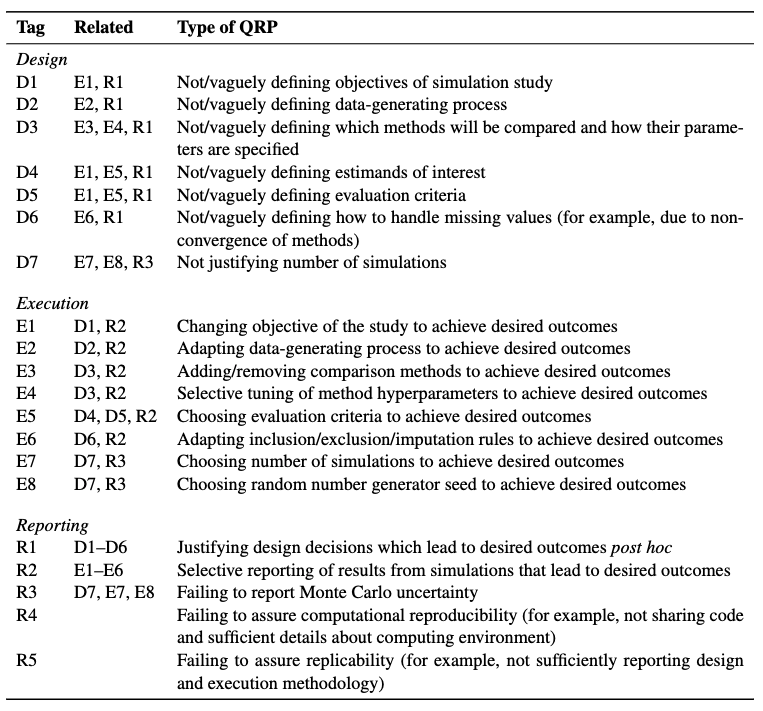
\includegraphics[scale=0.5]{Figures/screenshots/QRPSUMMARY.png}
	\caption{shows the outline of QRP classes and instances}
\end{figure}

\subsubsection{Applied examples of simulation studies}

[6] evaluated and compared the effectiveness of Cox regression analysis (CRA) and random survival forests (RSF) through both simulated and actual breast cancer data scenarios. Initially, the study utilised Monte Carlo simulations to assess how both methods performed across various sample sizes, specifically observing their performance metrics based on Harrell’s concordance index. The results indicated that CRA consistently outperformed RSF under simulation conditions, particularly when using the concordance index for evaluation. Following the simulations, the methods were applied to a real dataset comprising 279 breast cancer patients to identify major risk factors influencing disease-free survival (DFS). In this practical application, RSF slightly edged out other methods, offering marginally better performance according to the concordance index when using the approximate log-rank splitting rule.

Approximate log-rank splitting rule
% ### Formula

CRA was noted for its predictive accuracy across different sample sizes, making it suitable for a broad range of survival data applications. Conversely, RSF was recommended for its interpretative power, especially beneficial in handling complex datasets where multiple survival trees are analysed. [6]

Furthermore, [7] shows a comparison between a machine learning method, termed survival neural networks (SNNs) and compared it with the Cox proportional hazards model, using clinical trial data for survival outcomes. The models are formulated subject to the European Osteosarcoma intergroup trial data, which is used as the foundation for the synthetic data generation that would ultimately be used for simulation training. The original dataset contains various instances of censoring, and the authors approach this issue, by segmenting the
datasets into samples with degrees of censoring present (20%, 40%, 61%, 80%), afterwhich data imputation techniques such as the inverse probability weighting, censoring method (IPW), was used, which is based on calibration procedures outlined in the paper, to ensure the synthetic data retains the statistical properties of the original clinical data. The architecture used: 

% ### FORMULA

where j = 1, 2, . . . , J are the nodes in the input layer, h = 1, 2, . . . ,
H are the nodes in the hidden layer, and w are the weights of the network. The
training is performed with training sets and validation sets, using cross-validation and
hyperparameter tuning. Furthermore, evaluation techniques are explored, specifically
looking at factors like discrimination (C-index) by using the average time dependant
nonlinear prognostic index,

% ###FORMULA

Accuracy (Brier) interpreted in continuous form as the integrated Brier score for prediction error over the total period,

% ###FORMULA

And lastly Miscalibration (mean squared error) for censored groups. The results indicated comparable predictive performance but highlighted a lack of accuracy for calibration measures with SNNs. The authors point out that although machine learning techniques are attractive for survival analysis scenarios because of the ability to model interactions and nonlinearities with a no assumption approach, the robustness of the Cox model, regarding ease of implementation as well as interpretability of covariates makes it formidable in situations where limited sample sizes and variables are available. The paper ties in nicely with the other literature in support of the need for clear and better implementation of calibration metrics specifically with machine learning models, and caution against indiscriminate application of these models.

\subsection{Cox's Proportional Hazards Model}

\noindent
In the seminal work by [8], the cox model is introduced as an extension to prior work formalised as the Kaplan-Meier estimator, by exploring time-to-event data (life tables). The major benefit is that it addresses censored data, which is a known concept in survival analysis, that there is missing information within the data, specifically, event occurrence without observation on a continuous time scale. The proposition consists of covariates, known as attributes regarding a unit in a distribution of data, which is associated with a coefficient \(\beta\) scaling the impact of said covariates; this product is then bound by the baseline hazard h0(t).

%  ###FORMULA

Hazard being the estimated conditional probabilities, in line with the observed conditional frequencies of events or simply the risk of event occurrence at a specific time. An assumption of the Cox model is the proportional hazards assumption, suggesting that the hazard ratios for different covariates remain constant over time we see this for two events observations,

% ### FORMULA

This is an operational Assumption and a limitation as this is not always true for survival data. The model can handle censoring, by adjusting the likelihood function for observations where event occurrence did not happen in a particular continuous time frame, and by maximising the likelihood of all observed events, it is possible to estimate the coefficients that could work the best under the Cox formulation.

% ### FORMULA

\subsubsection{Time-Dependant Covariates}
\noindent
The Cox model incorporates both time-independent and time-dependent covariates. Time-dependent covariates can change over the time, such as Z2(t) = Z1*t. This flexibility allows the model to handle scenarios where hazards are not proportional, which extends its applicability. Relative risk is represented as exp(Z(t)'), showing how risk changes with time and covariate values and depending on the coefficients, the relative risk in a treatment group can increase, decrease, or remain constant over time. External covariates are variables that are independent of the subject’s survival process. Whereas internal covariates are variables that might influence and be influenced by survival. Different approaches for modelling survivor functions are required for external and internal covariates due to their nature.

\subsubsection{Discrete vs Continuous Model}
\noindent
Discrete Models address survival data that is categorical or not continuously distributed while the continuous model proposed by cox, utilises continuous data to model hazard functions. The survivor function can also be represented as a product integral which accommodates both discrete and continuous survival data. This approach allows for the unified handling of mixed data types in survival analysis. For the continuous model, estimation is based on maximising the conditional likelihood across observed failure times, while the discrete model uses a logistic framework for estimation, treating survival as a sequence of binary outcomes.

\subsubsection{Likelihood Function}
The various approaches to the Cox model handle data ties and time-dependent covariates differently, ….recommended specific methods based on the data structure (e.g., number of ties). The concept of partial likelihood is particularly important as it provides a way to focus on relevant factors in the presence of complex data types, enhancing both the theoretical understanding and practical application of the Cox model.

% The marginal likelihood approach (Kalbfleisch & Prentice, 1973), was developed for both uncensored and censored data. In uncensored scenarios, it treats the ranks of data points as arising from the marginal distribution, leading to the Cox likelihood. It allows for a statistical handling of tied data points by breaking ties in all possible ways, which though accurate, is computationally intensive. Breslow's step function approach (1974), assumes a step function for the baseline hazard with changes at observed failure times. Simplifies computations but is less theoretically satisfying as the model depends on the data itself. This approach is particularly useful for handling time-dependent covariates. Bailey's non-parametric approach (1984), which uses a nonparametric maximisation of the full likelihood. This provides estimators for regression coefficients and survival probabilities similar to those in previous methods. Finally the partial likelihood (Cox, 1975), that uses partial likelihood for estimation, separating the effect of nuisance parameters. This approach simplifies the computational process and can isolate useful data from noise

\subsection{Lasso Regularisation And Variable Selection}

\subsection{Random Surivival Forest}

\subsection{Methods For Data Generating Mechanisms For Simulation}

\subsection{Methods For Model Execution And Computation}

\subsection{Methods For Model Evaluation And Result Interpretation}



\section{Problem Statement}

\noindent 
Many studies have compared machine learning with traditional statistics, yet comprehensive simulation-based comparisons are scarce. This gap may lead to biases and sometimes questionable practices, affecting the validity of findings.

\section{Research Aims and Objectives}

\subsection{Research Aims}

\noindent 
Perform a comparative analysis of survival models using both simulated and real datasets to identify model robustness and effectiveness, adhering to formal frameworks and avoiding common pitfalls outlined in the literature.

\subsection{Objectives}

\begin{enumerate}
	\item Source a Practical Dataset: Acquire a dataset with clear metrics and pre-analyzed statistics for straightforward applicability in survival analysis. This dataset should comply with standards. 
	\item Dataset Analysis: Run analysis on dataset metrics and formulate appropriate data-generating methods to match distribution.
	\item Apply Data Generating Methods: Utilise standard libraries to generate simulated data that closely replicates the statistical properties of the real dataset.
	\item Construct Survival Models:
	\begin{enumerate}
		\item Random Survival Forest Model: Develop and apply this model using both the real and simulated datasets.
		\item Cox Proportional Hazards Model: Similarly, develop and apply this model with both datasets.
	\end{enumerate}
	\item Evaluate and Visualise Predictions: Use common survival analysis metrics for evaluation and employ visualisation tools from survival libraries to illustrate the results effectively.
\end{enumerate}
 
\section{Limitations}

Sed ullamcorper quam eu nisl interdum at interdum enim egestas. Aliquam placerat justo sed lectus lobortis ut porta nisl porttitor. Vestibulum mi dolor, lacinia molestie gravida at, tempus vitae ligula. Donec eget quam sapien, in viverra eros.

\par\vspace{0.5cm}
\noindent \Cshadowbox{
	\begin{minipage}{15cm}
		\medskip
		\color[rgb]{0.0,0.4,0.65}This section of the chapter addresses the scope of the research by identifying and discussing its limitations. These limitations might have a number of sources. For example, the size and extent of the data set used for the research could limit its generalisability. In this section, you should identify and discuss any such limitations that are foreseeable at the time of proposal.
		\medskip 
\end{minipage}}\\

\section{Assumptions and Definitions}

Morbi rutrum odio eget arcu adipiscing sodales. Aenean et purus a est pulvinar pellentesque.Cras in elit neque,  quis varius elit. Phasellus fringilla,  nibh eu tempus venenatis,  dolor elitposuere quam, quis adipiscing urna leo nec orci.  

\par\vspace{0.5cm}
\noindent \Cshadowbox{
	\begin{minipage}{15cm}
		\bigskip
		\color[rgb]{0.0,0.4,0.65} Like the section above, this section addresses the scope of the research, along with providing any relevant technical definitions from the literature. It should include the following.
			\begin{description}
				\item[Assumptions] Identify and discuss any notable assumptions of the research.
				\item[Definitions] Define any important technical terms appearing in the research.
			\end{description}
		\medskip 
\end{minipage}}\\

\section{Overview}
\noindent
In addressing the noted shortcomings in comparative simulation studies, this literature review methodically examines simulation work in segments relevant to each section of the study. We begin with an overview of the Cox method and its various extensions, illustrating how these foundational techniques are implemented. Following that, we explore proofs and extensions of the Lasso method, which build on the base Cox method, enhancing its predictive power and flexibility. The discussion then moves to Random Survival Forests (RSF), detailing recent advancements in RSF algorithms that provide a solid reference for current implementations. Two comparative studies are highlighted; these utilise simulations to evaluate the methods mentioned above, offering insights into their practical applications and effectiveness. Finally the last section categorises the literature into subgroups that align with the specific components of the proposed research framework….., facilitating easy reference and integration into the research design and methodology in Chapter 2, ensuring a coherent and structured approach to applying these methods in proposed study.
